\documentclass[12pt,]{article}
\usepackage{lmodern}
\usepackage{amssymb,amsmath}
\usepackage{ifxetex,ifluatex}
\usepackage{fixltx2e} % provides \textsubscript
\ifnum 0\ifxetex 1\fi\ifluatex 1\fi=0 % if pdftex
  \usepackage[T1]{fontenc}
  \usepackage[utf8]{inputenc}
\else % if luatex or xelatex
  \ifxetex
    \usepackage{mathspec}
  \else
    \usepackage{fontspec}
  \fi
  \defaultfontfeatures{Ligatures=TeX,Scale=MatchLowercase}
    \setmonofont[Mapping=tex-ansi,Scale=0.7]{Source Code Pro}
\fi
% use upquote if available, for straight quotes in verbatim environments
\IfFileExists{upquote.sty}{\usepackage{upquote}}{}
% use microtype if available
\IfFileExists{microtype.sty}{%
\usepackage{microtype}
\UseMicrotypeSet[protrusion]{basicmath} % disable protrusion for tt fonts
}{}
\usepackage[margin=1in]{geometry}
\usepackage{hyperref}
\PassOptionsToPackage{usenames,dvipsnames}{color} % color is loaded by hyperref
\hypersetup{unicode=true,
            pdftitle={Biostatistics using R},
            pdfauthor={Dewey Brooke},
            colorlinks=true,
            linkcolor=Maroon,
            citecolor=Blue,
            urlcolor=Blue,
            breaklinks=true}
\urlstyle{same}  % don't use monospace font for urls
\usepackage{natbib}
\bibliographystyle{apalike}
\usepackage{color}
\usepackage{fancyvrb}
\newcommand{\VerbBar}{|}
\newcommand{\VERB}{\Verb[commandchars=\\\{\}]}
\DefineVerbatimEnvironment{Highlighting}{Verbatim}{commandchars=\\\{\}}
% Add ',fontsize=\small' for more characters per line
\usepackage{framed}
\definecolor{shadecolor}{RGB}{248,248,248}
\newenvironment{Shaded}{\begin{snugshade}}{\end{snugshade}}
\newcommand{\AlertTok}[1]{\textcolor[rgb]{0.94,0.16,0.16}{#1}}
\newcommand{\AnnotationTok}[1]{\textcolor[rgb]{0.56,0.35,0.01}{\textbf{\textit{#1}}}}
\newcommand{\AttributeTok}[1]{\textcolor[rgb]{0.77,0.63,0.00}{#1}}
\newcommand{\BaseNTok}[1]{\textcolor[rgb]{0.00,0.00,0.81}{#1}}
\newcommand{\BuiltInTok}[1]{#1}
\newcommand{\CharTok}[1]{\textcolor[rgb]{0.31,0.60,0.02}{#1}}
\newcommand{\CommentTok}[1]{\textcolor[rgb]{0.56,0.35,0.01}{\textit{#1}}}
\newcommand{\CommentVarTok}[1]{\textcolor[rgb]{0.56,0.35,0.01}{\textbf{\textit{#1}}}}
\newcommand{\ConstantTok}[1]{\textcolor[rgb]{0.00,0.00,0.00}{#1}}
\newcommand{\ControlFlowTok}[1]{\textcolor[rgb]{0.13,0.29,0.53}{\textbf{#1}}}
\newcommand{\DataTypeTok}[1]{\textcolor[rgb]{0.13,0.29,0.53}{#1}}
\newcommand{\DecValTok}[1]{\textcolor[rgb]{0.00,0.00,0.81}{#1}}
\newcommand{\DocumentationTok}[1]{\textcolor[rgb]{0.56,0.35,0.01}{\textbf{\textit{#1}}}}
\newcommand{\ErrorTok}[1]{\textcolor[rgb]{0.64,0.00,0.00}{\textbf{#1}}}
\newcommand{\ExtensionTok}[1]{#1}
\newcommand{\FloatTok}[1]{\textcolor[rgb]{0.00,0.00,0.81}{#1}}
\newcommand{\FunctionTok}[1]{\textcolor[rgb]{0.00,0.00,0.00}{#1}}
\newcommand{\ImportTok}[1]{#1}
\newcommand{\InformationTok}[1]{\textcolor[rgb]{0.56,0.35,0.01}{\textbf{\textit{#1}}}}
\newcommand{\KeywordTok}[1]{\textcolor[rgb]{0.13,0.29,0.53}{\textbf{#1}}}
\newcommand{\NormalTok}[1]{#1}
\newcommand{\OperatorTok}[1]{\textcolor[rgb]{0.81,0.36,0.00}{\textbf{#1}}}
\newcommand{\OtherTok}[1]{\textcolor[rgb]{0.56,0.35,0.01}{#1}}
\newcommand{\PreprocessorTok}[1]{\textcolor[rgb]{0.56,0.35,0.01}{\textit{#1}}}
\newcommand{\RegionMarkerTok}[1]{#1}
\newcommand{\SpecialCharTok}[1]{\textcolor[rgb]{0.00,0.00,0.00}{#1}}
\newcommand{\SpecialStringTok}[1]{\textcolor[rgb]{0.31,0.60,0.02}{#1}}
\newcommand{\StringTok}[1]{\textcolor[rgb]{0.31,0.60,0.02}{#1}}
\newcommand{\VariableTok}[1]{\textcolor[rgb]{0.00,0.00,0.00}{#1}}
\newcommand{\VerbatimStringTok}[1]{\textcolor[rgb]{0.31,0.60,0.02}{#1}}
\newcommand{\WarningTok}[1]{\textcolor[rgb]{0.56,0.35,0.01}{\textbf{\textit{#1}}}}
\usepackage{longtable,booktabs}
\usepackage{graphicx,grffile}
\makeatletter
\def\maxwidth{\ifdim\Gin@nat@width>\linewidth\linewidth\else\Gin@nat@width\fi}
\def\maxheight{\ifdim\Gin@nat@height>\textheight\textheight\else\Gin@nat@height\fi}
\makeatother
% Scale images if necessary, so that they will not overflow the page
% margins by default, and it is still possible to overwrite the defaults
% using explicit options in \includegraphics[width, height, ...]{}
\setkeys{Gin}{width=\maxwidth,height=\maxheight,keepaspectratio}
\IfFileExists{parskip.sty}{%
\usepackage{parskip}
}{% else
\setlength{\parindent}{0pt}
\setlength{\parskip}{6pt plus 2pt minus 1pt}
}
\setlength{\emergencystretch}{3em}  % prevent overfull lines
\providecommand{\tightlist}{%
  \setlength{\itemsep}{0pt}\setlength{\parskip}{0pt}}
\setcounter{secnumdepth}{5}
% Redefines (sub)paragraphs to behave more like sections
\ifx\paragraph\undefined\else
\let\oldparagraph\paragraph
\renewcommand{\paragraph}[1]{\oldparagraph{#1}\mbox{}}
\fi
\ifx\subparagraph\undefined\else
\let\oldsubparagraph\subparagraph
\renewcommand{\subparagraph}[1]{\oldsubparagraph{#1}\mbox{}}
\fi

%%% Use protect on footnotes to avoid problems with footnotes in titles
\let\rmarkdownfootnote\footnote%
\def\footnote{\protect\rmarkdownfootnote}

%%% Change title format to be more compact
\usepackage{titling}

% Create subtitle command for use in maketitle
\newcommand{\subtitle}[1]{
  \posttitle{
    \begin{center}\large#1\end{center}
    }
}

\setlength{\droptitle}{-2em}

  \title{Biostatistics using R}
    \pretitle{\vspace{\droptitle}\centering\huge}
  \posttitle{\par}
    \author{Dewey Brooke}
    \preauthor{\centering\large\emph}
  \postauthor{\par}
      \predate{\centering\large\emph}
  \postdate{\par}
    \date{2018-08-30}


\begin{document}
\maketitle

{
\hypersetup{linkcolor=black}
\setcounter{tocdepth}{2}
\tableofcontents
}
\listoftables
\listoffigures
\hypertarget{preface}{%
\section*{Preface}\label{preface}}
\addcontentsline{toc}{section}{Preface}

This is a \emph{sample} book written in \textbf{Markdown}. You can use
anything that Pandoc's Markdown supports, e.g., a math equation
\(a^2 + b^2 = c^2\).

The \textbf{bookdown} package can be installed from CRAN or Github:

\begin{Shaded}
\begin{Highlighting}[]
\KeywordTok{install.packages}\NormalTok{(}\StringTok{"bookdown"}\NormalTok{)}
\CommentTok{# or the development version}
\CommentTok{# devtools::install_github("rstudio/bookdown")}
\end{Highlighting}
\end{Shaded}

Remember each Rmd file contains one and only one chapter, and a chapter
is defined by the first-level heading \texttt{\#}.

To compile this example to PDF, you need XeLaTeX. You are recommended to
install TinyTeX (which includes XeLaTeX):
\url{https://yihui.name/tinytex/}.

\hypertarget{intro}{%
\section{Introduction}\label{intro}}

\hypertarget{reading-data-files-into-r}{%
\subsection*{Reading Data Files into
R}\label{reading-data-files-into-r}}
\addcontentsline{toc}{subsection}{Reading Data Files into R}

The first step in every analysis requires data to be read into the
environment, and learning how to do this is the first hurdle a person
needs to overcome to begin learning to use R.

Data can exist in many different formats, either as the generic
universal types (e.g.~csv, tsv, .json, etc) or software specific types
(e.g. \texttt{.xlsx}, `` )

In this chapter, we will first discuss how to read data using functions
in Base-R (when possible), and then we will discuss alternative
packages, such as the multitude of packages in the
\href{https://www.tidyverse.org}{Tidyverse}, and highlight their
advantages over Base-R functions.

\hypertarget{generic-formats}{%
\subsubsection{Generic Formats}\label{generic-formats}}

\hypertarget{csv--comma-separated-values}{%
\paragraph{CSV- Comma Separated
Values}\label{csv--comma-separated-values}}

The fields are separated by a comma \texttt{,} and are typically used
for loading into spreadsheets.

For example:

\begin{Shaded}
\begin{Highlighting}[]
\NormalTok{csv_example_path <-}\StringTok{ "data/ASCII-comma/FEV.DAT.txt"}

\KeywordTok{readLines}\NormalTok{(csv_example_path)[}\DecValTok{1}\OperatorTok{:}\DecValTok{8}\NormalTok{]  }\CommentTok{# reads each line of the file}
\end{Highlighting}
\end{Shaded}

\begin{verbatim}
[1] "'Id','Age','FEV','Hgt','Sex','Smoke'"
[2] "301,9,1.708,57,0,0"                  
[3] "451,8,1.724,67.5,0,0"                
[4] "501,7,1.72,54.5,0,0"                 
[5] "642,9,1.558,53,1,0"                  
[6] "901,9,1.895,57,1,0"                  
[7] "1701,8,2.336,61,0,0"                 
[8] "1752,6,1.919,58,0,0"                 
\end{verbatim}

\begin{Shaded}
\begin{Highlighting}[]
\CommentTok{# Note: readLines(csv_example_path) is the same as}
\CommentTok{# readLines("data/ASCII-comma/FEV.DAT.txt")}
\end{Highlighting}
\end{Shaded}

In Base-R, CSV data can be read using the \texttt{read.csv()} function.
The \texttt{read.csv2()} function is used in countries that use a comma
as a decimal point and a semicolon as a field separator.

\begin{Shaded}
\begin{Highlighting}[]
\NormalTok{csv_example <-}\StringTok{ }\KeywordTok{read.csv}\NormalTok{(csv_example_path)}

\KeywordTok{head}\NormalTok{(csv_example)}
\end{Highlighting}
\end{Shaded}

\begin{verbatim}
  X.Id. X.Age. X.FEV. X.Hgt. X.Sex. X.Smoke.
1   301      9  1.708   57.0      0        0
2   451      8  1.724   67.5      0        0
3   501      7  1.720   54.5      0        0
4   642      9  1.558   53.0      1        0
5   901      9  1.895   57.0      1        0
6  1701      8  2.336   61.0      0        0
\end{verbatim}

\hypertarget{tsv--tab-separated-values}{%
\paragraph{TSV- Tab Separated Values}\label{tsv--tab-separated-values}}

The fields are separated by a tabulation or \t and are saved as
\texttt{.txt} files. However, not all \texttt{.txt} files contain tab
separated values.

For example:

\begin{Shaded}
\begin{Highlighting}[]
\NormalTok{tsv_example_path <-}\StringTok{ "data/ASCII-tab/FEV.DAT.txt"}

\KeywordTok{readLines}\NormalTok{(tsv_example_path)[}\DecValTok{1}\OperatorTok{:}\DecValTok{8}\NormalTok{]}
\end{Highlighting}
\end{Shaded}

\begin{verbatim}
[1] "'Id'\t'Age'\t'FEV'\t'Hgt'\t'Sex'\t'Smoke'"
[2] "301\t9\t1.708\t57\t0\t0"                  
[3] "451\t8\t1.724\t67.5\t0\t0"                
[4] "501\t7\t1.72\t54.5\t0\t0"                 
[5] "642\t9\t1.558\t53\t1\t0"                  
[6] "901\t9\t1.895\t57\t1\t0"                  
[7] "1701\t8\t2.336\t61\t0\t0"                 
[8] "1752\t6\t1.919\t58\t0\t0"                 
\end{verbatim}

\begin{Shaded}
\begin{Highlighting}[]
\NormalTok{tsv_example <-}\StringTok{ }\KeywordTok{read.delim}\NormalTok{(}\StringTok{"data/ASCII-tab/FEV.DAT.txt"}\NormalTok{)}
\KeywordTok{head}\NormalTok{(tsv_example)}
\end{Highlighting}
\end{Shaded}

\begin{verbatim}
  X.Id. X.Age. X.FEV. X.Hgt. X.Sex. X.Smoke.
1   301      9  1.708   57.0      0        0
2   451      8  1.724   67.5      0        0
3   501      7  1.720   54.5      0        0
4   642      9  1.558   53.0      1        0
5   901      9  1.895   57.0      1        0
6  1701      8  2.336   61.0      0        0
\end{verbatim}

\hypertarget{excel}{%
\subsubsection{Excel}\label{excel}}

\begin{Shaded}
\begin{Highlighting}[]
\KeywordTok{library}\NormalTok{(readxl)}
\end{Highlighting}
\end{Shaded}

\hypertarget{software-specific-formats}{%
\subsubsection{Software Specific
Formats}\label{software-specific-formats}}

R is increasingly recognized as the gold standard for statistical
computations, yet some of your future collaborates will exclusively use
Commercial Software (SAS, SPSS, Matlab, and Stata) for their statistical
computations. Although these individuals are limited by the types of
files they can read or write, the \texttt{haven} R-package can both read
and write any of these file formats.

\begin{Shaded}
\begin{Highlighting}[]
\KeywordTok{library}\NormalTok{(haven)}
\end{Highlighting}
\end{Shaded}

\hypertarget{sas.sas7bdat-spss.sav.por-.xpt-stata-.dta}{%
\paragraph{\texorpdfstring{SAS(\texttt{.sas7bdat}),
SPSS(\texttt{.sav},\texttt{.por}, \texttt{.xpt}), Stata
(\texttt{.dta})}{SAS(.sas7bdat), SPSS(.sav,.por, .xpt), Stata (.dta)}}\label{sas.sas7bdat-spss.sav.por-.xpt-stata-.dta}}

\begin{Shaded}
\begin{Highlighting}[]
\NormalTok{sas <-}\StringTok{ }\KeywordTok{read_sas}\NormalTok{(}\StringTok{"data/SAS/FEV.sas7bdat"}\NormalTok{)}

\KeywordTok{head}\NormalTok{(sas)}
\end{Highlighting}
\end{Shaded}

\begin{verbatim}
# A tibble: 6 x 6
     ID   AGE   FEV   HGT   SEX SMOKE
  <dbl> <dbl> <dbl> <dbl> <dbl> <dbl>
1   301     9  1.71  57       0     0
2   451     8  1.72  67.5     0     0
3   501     7  1.72  54.5     0     0
4   642     9  1.56  53       1     0
5   901     9  1.90  57       1     0
6  1701     8  2.34  61       0     0
\end{verbatim}

\begin{Shaded}
\begin{Highlighting}[]
\NormalTok{spss <-}\StringTok{ }\KeywordTok{read_spss}\NormalTok{(}\StringTok{"data/SPSS/FEV.DAT.sav"}\NormalTok{)}
\KeywordTok{head}\NormalTok{(spss)}
\end{Highlighting}
\end{Shaded}

\begin{verbatim}
# A tibble: 6 x 6
     Id   Age   FEV   Hgt   Sex Smoke
  <dbl> <dbl> <dbl> <dbl> <dbl> <dbl>
1   301     9  1.71  57       0     0
2   451     8  1.72  67.5     0     0
3   501     7  1.72  54.5     0     0
4   642     9  1.56  53       1     0
5   901     9  1.90  57       1     0
6  1701     8  2.34  61       0     0
\end{verbatim}

\begin{Shaded}
\begin{Highlighting}[]
\NormalTok{stata <-}\StringTok{ }\KeywordTok{read_stata}\NormalTok{(}\StringTok{"data/Stata/FEV.DAT.dta"}\NormalTok{)}
\KeywordTok{head}\NormalTok{(stata)}
\end{Highlighting}
\end{Shaded}

\begin{verbatim}
# A tibble: 6 x 6
     Id   Age   fev   Hgt   Sex Smoke
  <dbl> <dbl> <dbl> <dbl> <dbl> <dbl>
1   301     9  1.71  57       0     0
2   451     8  1.72  67.5     0     0
3   501     7  1.72  54.5     0     0
4   642     9  1.56  53       1     0
5   901     9  1.90  57       1     0
6  1701     8  2.34  61       0     0
\end{verbatim}

The \texttt{foreign} package included in Base-R can also be used to
Reading and writing data stored by some versions of `Epi Info',
`Minitab', `S', `SAS', `SPSS', `Stata', `Systat', `Weka',and for reading
and writing some `dBase' files.

RDS

\begin{Shaded}
\begin{Highlighting}[]
\NormalTok{rds_example <-}\StringTok{ }\KeywordTok{readRDS}\NormalTok{(}\StringTok{"data/RDS/BETACAR.DAT.rds"}\NormalTok{)}
\KeywordTok{head}\NormalTok{(rds_example)}
\end{Highlighting}
\end{Shaded}

\begin{verbatim}
# A tibble: 6 x 8
  `'Prepar'` `'Id'` `'Base1lvl'` `'Base2lvl'`
       <int>  <int>        <int>        <int>
1          1     71          298          116
2          1     73          124          146
3          1     80          176          200
4          1     83          116          180
5          1     90          152          142
6          1     92          106          106
# ... with 4 more variables: `'Wk6lvl'` <int>,
#   `'Wk8lvl'` <int>, `'Wk10lvl'` <int>,
#   `'Wk12lvl'` <int>
\end{verbatim}

\texttt{rdata}

The \texttt{.rdata} format is R's specific format. Instead of using a
\texttt{read.\{something\}} function, \texttt{.rdata} is read into the
environment using \texttt{load(filename.rdata)} and retains the original
name it had when it was last saved.

\begin{Shaded}
\begin{Highlighting}[]
\KeywordTok{load}\NormalTok{(}\StringTok{"data/R/BETACAR.DAT.rdata"}\NormalTok{)  }\CommentTok{#named betacar when it was last saved}
\KeywordTok{head}\NormalTok{(betacar)}
\end{Highlighting}
\end{Shaded}

\begin{verbatim}
  Prepar Id Base1lvl Base2lvl Wk6lvl Wk8lvl Wk10lvl
1      1 71      298      116    174    178     218
2      1 73      124      146    294    278     244
3      1 80      176      200    276    286     308
4      1 83      116      180    164    238     308
5      1 90      152      142    290    300     270
6      1 92      106      106    246    206     304
  Wk12lvl
1     190
2     262
3     334
4     226
5     268
6     356
\end{verbatim}

\hypertarget{descriptive-statistics}{%
\section{Descriptive Statistics}\label{descriptive-statistics}}

\begin{verbatim}
PhantomJS not found. You can install it with webshot::install_phantomjs(). If it is installed, please make sure the phantomjs executable can be found via the PATH variable.
\end{verbatim}

\hypertarget{htmlwidget-0b4418012763d828a34d}{}

\hypertarget{introduction-to-probablity}{%
\subsection{Introduction to
Probablity}\label{introduction-to-probablity}}

\hypertarget{definitions}{%
\subsubsection{Definitions}\label{definitions}}

\textbf{Sample Space}: set of all possible outcomes in an experiment or
trial

\textbf{Event}: any individual outcome of interest, or subset of
outcomes of interest, in an experiment or trial

\textbf{Probablity}: relative frequency of an event of interest over an
indefintely large (or infinite) number of trials

\hypertarget{probablity}{%
\subsubsection{Probablity}\label{probablity}}

The true probablity of an event is often unknown and ca only be
estimated.

\textbf{Relative frequency probablity}: Counting the number of
repetitions of a process and the number of times each events occurs -
Divide the number of each outcome by the total number of repetitions -
This estimates the likelihood of each event occuring -This follows the
ideas of bar charts and histograms

\hypertarget{sampling}{%
\subsubsection{Sampling}\label{sampling}}

\textbf{Population}: A well defined collection of objects, such as:
pregnant women, MS patients, stroke survivors, etc. - Measurements on
every member of th population consitutes a census. - A census may not be
feasible or desired.

\textbf{Sample}: a subset of the populaiton from which characterstics
are measured in order to estimate and infer characteristics of the
population. - Individual components of the sample are its elements
(observations)

\hypertarget{statistics}{%
\subsubsection{Statistics}\label{statistics}}

\textbf{Parameters}: fixed values used to describe characteristics of a
variable's distribution (e.g., where it is centered, measures of its
spread, measures of its skewness, etc.)

Common paramters are the mean and standard deviation.

Go back and fix ***

\hypertarget{descriptive-statistics-summary-statistics-used-to-estiamte-population-paramters}{%
\subsubsection{\texorpdfstring{\textbf{Descriptive Statistics:} summary
statistics used to estiamte population
paramters}{Descriptive Statistics: summary statistics used to estiamte population paramters}}\label{descriptive-statistics-summary-statistics-used-to-estiamte-population-paramters}}

Sample statistics include \(\bar{x}, s^2, s\) - lower case letters are
used for describing samples.

Population parameters are estimated from the sample - population
parameters include \(\mu, \sigma^s, \sigma\)

Inferential Statistics

Go back and fix ***

\hypertarget{describing-data}{%
\paragraph{Describing Data}\label{describing-data}}

Data are summarized by descriptive statistics, and distributions of
variables are often depicted using plots including: -charts -histograms

go back and fix ***

Of we have a sample of n objects, then the values are denoted as
\(x_1, x_2, ..., x_n\).

The sample mean \[\bar{x} = \frac{\sum_i^nx}{n}\]

Sample variance \(s^2 = \frac{\sum_i^n{x_i-\bar{x}}}{n-1}\)

Sample std dev \(s = \sqrt{s^2}\)

It can be shown that \(\sum{x_i-\bar{x}}=0\) and the actual differences
between each observation and the samle mean are not informative.

The square distance between the observed values and the sample mean is
what we examine.

Alternative measure is the \textbf{mean obsolute deviation} (MAD)
\[\text{MAD} = \frac{\sum^n_{i=1}|x_i-\bar{x}|}{n}\]

\textbf{Median}: the middle value in the list of ordered values (the
median is the \(50^\text{th}\) percentile)

\textbf{Percentile}: the value such that some percent of the data are
less than that value. - for the ordered data, the \(k^\text{th}\)
percentile is in the \(\frac{k}{100}(1+n)\) position. - if the position
falls between 2 numbers, then the \(k^\text{th}\) percentile is the
average of the two surrounding numbers.

\textbf{quartiles}: the \(25^\text{th}\) (\(Q_1\)) and \(75^\text{th}\)
(\(Q_3\))

\textbf{interquartile range}: \(75^\text{th}-50^\text{th}\) percentile

\hypertarget{measures-of-location-using-base-r}{%
\subsection{Measures of Location using Base
R}\label{measures-of-location-using-base-r}}

\begin{quote}
Determining the correct method for measuring the central tendancy of a
vector depends on the relationship between the numbers within the
vector. Numbers that can be summed in a linear sequence are best
represented using the arithmic mean.

If you're measuring units that add up as reciprocals in a sequence (such
as speed or distance / time over a constant distance, capacitance in
series, resistance in parallel), then a harmonic mean will give you a
meaningful average. For example, the harmonic mean of capacitors in
series represents the capacitance that a single capacitor would have if
only one capacitor was used instead of the set of capacitors in series.

If you're measuring units that multiply in a sequence (such as growth
rates or percentages), then a geometric mean will give you a meaningful
average. For example, the geometric mean of a sequence of different
annual interest rates over 10 years represents an interest rate that, if
applied constantly for ten years, would produce the same amount growth
in principal as the sequence of different annual interest rates over ten
years did. Does an arithmetic mean of interest rates have any
significance? As a number, sure. But as an ``average'' interest rate it
seems less intuitive because the principal it produces at the end of ten
years is much larger than the geometric mean. Similarly, the harmonic
mean of interest rates produces a smaller principal, and so is less
intuitive.

Now consider areas and volumes as a test of understanding. What mean
should we use to report the ``average'' area or volume in a sequence of
areas or volumes? Area is measured in units of length squared. Volume is
measured in units of length cubed. In a sequence of areas or volumes, we
could either add them up linearly and divide or multiply them and take
the roots --- which is correct? It depends on what we're measuring. If
these areas or volumes are dependent upon each other (e.g., the size of
the same microbe at different times), then a geometric mean probably
makes more sense. If these areas or volumes are independent of each
other (e.g., the size of a house or pool), then an arithmetic mean
probably makes more sense. But whatever you decide, when in doubt report
that decision. There is nothing worse for a reader than to see an
``average'' and not know how it was calculated! -
\href{https://www.quora.com/When-is-it-most-appropriate-to-take-the-arithmetic-mean-vs-geometric-mean-vs-harmonic-mean}{Michael
F. Martin,Quora Answer}
\end{quote}

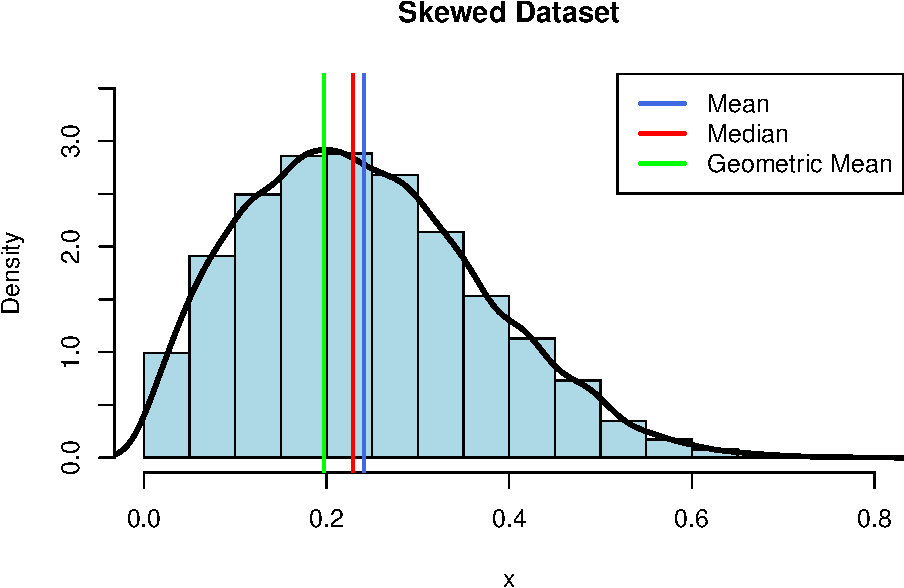
\includegraphics{bst4r_files/figure-latex/unnamed-chunk-12-1.pdf}

\hypertarget{the-arithmetic-mean}{%
\subsubsection{The Arithmetic Mean}\label{the-arithmetic-mean}}

The arithmetic mean is the sum of all the observations divided by the
number of observations. It is written in statistical terms as

\[\overline{x} = \frac{1}{n}\sum^n_{i=1}x_i\]

\begin{Shaded}
\begin{Highlighting}[]
\KeywordTok{mean}\NormalTok{(ChickWeight}\OperatorTok{$}\NormalTok{weight)}
\end{Highlighting}
\end{Shaded}

\begin{verbatim}
[1] 121.8
\end{verbatim}

\hypertarget{the-median}{%
\subsubsection{The Median}\label{the-median}}

The sample median is:

\begin{enumerate}
\def\labelenumi{\arabic{enumi}.}
\item
  If \emph{n} is odd \(\rightarrow\)
  \(\Big(\frac{n+1}{2}\Big)\text{th}\) largest observation
\item
  If \emph{n} is even \(\rightarrow\) \(\Big(\frac{n}{2}\Big)\text{th}\)
  and \(\Big(\frac{n}{2}+1\Big)\text{th}\) largest observations
\end{enumerate}

\begin{Shaded}
\begin{Highlighting}[]
\KeywordTok{median}\NormalTok{(ChickWeight}\OperatorTok{$}\NormalTok{weight)}
\end{Highlighting}
\end{Shaded}

\begin{verbatim}
[1] 103
\end{verbatim}

\hypertarget{the-mode}{%
\subsubsection{The Mode}\label{the-mode}}

The mode is the most frequently occurring value among all observations
in the sample. Although it is infrequently used, it is very useful for
categorical and discrete data.

Since there isn't a built in R-function for mode, we learn how to write
a function to return the mode through a few examples.

\hypertarget{functions}{%
\paragraph{Functions}\label{functions}}

\begin{center}\rule{0.5\linewidth}{\linethickness}\end{center}

\hypertarget{base-r-example}{%
\subparagraph{Base R Example}\label{base-r-example}}

The most simple function begins by assigning the output of
\texttt{function()} to some character string (e.g. \texttt{simple\_fun})

All statements after the \texttt{function()} are referred as the body of
the function.

\begin{Shaded}
\begin{Highlighting}[]
\NormalTok{function_name <-}\StringTok{ }\ControlFlowTok{function}\NormalTok{(arg1, arg2,...) \{}
  \CommentTok{#statements}
  
  \KeywordTok{return}\NormalTok{(}\StringTok{"some output"}\NormalTok{)}
\NormalTok{\}}
\KeywordTok{function_name}\NormalTok{() }\CommentTok{# returns NULL}
\end{Highlighting}
\end{Shaded}

\begin{verbatim}
[1] "some output"
\end{verbatim}

Use \texttt{return()} to output the result of the function.

\begin{Shaded}
\begin{Highlighting}[]
\NormalTok{return_value <-}\StringTok{ }\ControlFlowTok{function}\NormalTok{(x,y) \{}
\NormalTok{  z=x}\OperatorTok{-}\NormalTok{y  }
\NormalTok{  z=x}\OperatorTok{+}\NormalTok{y}
  \KeywordTok{return}\NormalTok{(z)}
\NormalTok{\}}
\KeywordTok{return_value}\NormalTok{(}\DecValTok{4}\NormalTok{,}\DecValTok{5}\NormalTok{) }
\end{Highlighting}
\end{Shaded}

\begin{verbatim}
[1] 9
\end{verbatim}

Since our goal is to find the most frequently occurring value in our
data-set (\texttt{ChickWeight}), we need to decide the sequence of
functions that we need to accomplish this. As you continue to add
various R functions to your R tool belt, you will find many possible
combinations for the same solution.

First, let's assign the weight column from ChickWeight to x to simplify
things. When \texttt{x} is called, the weight column from ChickWeight is
returned as a vector.

\begin{Shaded}
\begin{Highlighting}[]
\NormalTok{x<-ChickWeight}\OperatorTok{$}\NormalTok{weight}
\KeywordTok{head}\NormalTok{(x)}
\end{Highlighting}
\end{Shaded}

\begin{verbatim}
[1] 42 51 59 64 76 93
\end{verbatim}

We can return the size of \texttt{x} using the \texttt{length} function.
578

\begin{Shaded}
\begin{Highlighting}[]
\KeywordTok{length}\NormalTok{(x)}
\end{Highlighting}
\end{Shaded}

\begin{verbatim}
[1] 578
\end{verbatim}

We can reduce x to return only the unique values by using the
\texttt{unique} function. We'll assign it to y so we can use it later.

\begin{Shaded}
\begin{Highlighting}[]
\NormalTok{y <-}\StringTok{ }\KeywordTok{unique}\NormalTok{(x)}
\KeywordTok{length}\NormalTok{(y)}
\end{Highlighting}
\end{Shaded}

\begin{verbatim}
[1] 212
\end{verbatim}

To more easily watch how the functions are working, we will create two
data-frames to watch how we are manipulating both x and y.

\begin{Shaded}
\begin{Highlighting}[]
\NormalTok{df.x <-}\StringTok{ }\KeywordTok{data.frame}\NormalTok{(x)}
\NormalTok{df.y <-}\StringTok{ }\KeywordTok{data.frame}\NormalTok{(y)}
\end{Highlighting}
\end{Shaded}

Using the unique values from the \texttt{x} vector we defined as
\texttt{y}, we can use the \texttt{match} function to return a vector
that replaces each value in x with their position in the y vector
(1-212).

\begin{Shaded}
\begin{Highlighting}[]
\NormalTok{df.x}\OperatorTok{$}\NormalTok{position_in_y<-}\KeywordTok{match}\NormalTok{(x, y)}
\KeywordTok{head}\NormalTok{(df.x, }\DataTypeTok{n =} \DecValTok{30}\NormalTok{)}
\end{Highlighting}
\end{Shaded}

\begin{verbatim}
     x position_in_y
1   42             1
2   51             2
3   59             3
4   64             4
5   76             5
6   93             6
7  106             7
8  125             8
9  149             9
10 171            10
11 199            11
12 205            12
13  40            13
14  49            14
15  58            15
16  72            16
17  84            17
18 103            18
19 122            19
20 138            20
21 162            21
22 187            22
23 209            23
24 215            24
25  43            25
26  39            26
27  55            27
28  67            28
29  84            17
30  99            29
\end{verbatim}

The output from match can then be simplified using the tabulate function

\begin{Shaded}
\begin{Highlighting}[]
\NormalTok{df.y}\OperatorTok{$}\NormalTok{frequency <-}\StringTok{ }\KeywordTok{tabulate}\NormalTok{(df.x}\OperatorTok{$}\NormalTok{position_in_y)}
\KeywordTok{head}\NormalTok{(df.y)}
\end{Highlighting}
\end{Shaded}

\begin{verbatim}
   y frequency
1 42        15
2 51         8
3 59         5
4 64         5
5 76         3
6 93         4
\end{verbatim}

\texttt{which.max} returns the position of the maximum value.

\begin{Shaded}
\begin{Highlighting}[]
\KeywordTok{which.max}\NormalTok{(df.y}\OperatorTok{$}\NormalTok{frequency)}
\end{Highlighting}
\end{Shaded}

\begin{verbatim}
[1] 43
\end{verbatim}

\begin{Shaded}
\begin{Highlighting}[]
\NormalTok{df.y[}\DecValTok{43}\NormalTok{,]  }\CommentTok{#df.y[row,column]}
\end{Highlighting}
\end{Shaded}

\begin{verbatim}
    y frequency
43 41        20
\end{verbatim}

Putting it all together, we can do this in one line.

\begin{Shaded}
\begin{Highlighting}[]
\NormalTok{df.y[}\KeywordTok{which.max}\NormalTok{(}\KeywordTok{tabulate}\NormalTok{(}\KeywordTok{match}\NormalTok{(x,y))),] }
\end{Highlighting}
\end{Shaded}

\begin{verbatim}
    y frequency
43 41        20
\end{verbatim}

\begin{Shaded}
\begin{Highlighting}[]
\NormalTok{y[}\KeywordTok{which.max}\NormalTok{(}\KeywordTok{tabulate}\NormalTok{(}\KeywordTok{match}\NormalTok{(x,y)))]}
\end{Highlighting}
\end{Shaded}

\begin{verbatim}
[1] 41
\end{verbatim}

Writing this as a function

\begin{Shaded}
\begin{Highlighting}[]
\NormalTok{mode <-}\StringTok{ }\ControlFlowTok{function}\NormalTok{(x)\{}
\NormalTok{  unique_x <-}\StringTok{ }\KeywordTok{unique}\NormalTok{(x)}
\NormalTok{  result<-unique_x[}\KeywordTok{which.max}\NormalTok{(}\KeywordTok{tabulate}\NormalTok{(}\KeywordTok{match}\NormalTok{(x,unique_x)))]}
  \KeywordTok{return}\NormalTok{(result)}
\NormalTok{\}}

\KeywordTok{mode}\NormalTok{(x)}
\end{Highlighting}
\end{Shaded}

\begin{verbatim}
[1] 41
\end{verbatim}

\hypertarget{tidyverse-example}{%
\subparagraph{Tidyverse Example}\label{tidyverse-example}}

As with most problems in R, we can also find a solution using packages
from the Tidyverse. We will therefore use this as an opportunity to
introduce some of the basic tenants of Tidyverse functions.

In the \texttt{dplyr} package, a typical workflow will combine
observations into a single data-frame, aggregate them into groups,
manipulate values into new columns, and summaries the data-frame into
more simple terms.

The piping operator \texttt{\%\textgreater{}\%} allows for this to be
done seamlessly by literally pipping the result of one function into
arguments of another function.

\begin{Shaded}
\begin{Highlighting}[]
\KeywordTok{print}\NormalTok{(}\StringTok{"non-piped text"}\NormalTok{)}
\end{Highlighting}
\end{Shaded}

\begin{verbatim}
[1] "non-piped text"
\end{verbatim}

\begin{Shaded}
\begin{Highlighting}[]
\KeywordTok{library}\NormalTok{(dplyr)}
\StringTok{"piped text"} \OperatorTok\StringTok{ }\KeywordTok{print}\NormalTok{()}
\end{Highlighting}
\end{Shaded}

\begin{verbatim}
[1] "piped text"
\end{verbatim}

To show how this works, we will start with a simple example where we
first want to divided the sum of three and some other number (e.g.~2) by
seven.

Because of the order of operations, the sum of two and three would need
to be placed with parenthesis to indicate it happens before dividing by
seven.

\begin{Shaded}
\begin{Highlighting}[]
\NormalTok{(}\DecValTok{4}\OperatorTok{+}\DecValTok{3}\NormalTok{)}\OperatorTok{/}\DecValTok{7} \CommentTok{# correct}
\end{Highlighting}
\end{Shaded}

\begin{verbatim}
[1] 1
\end{verbatim}

\begin{Shaded}
\begin{Highlighting}[]
\DecValTok{4} \OperatorTok{+}\StringTok{ }\DecValTok{3} \OperatorTok{/}\StringTok{ }\DecValTok{7} \CommentTok{# incorrect}
\end{Highlighting}
\end{Shaded}

\begin{verbatim}
[1] 4.429
\end{verbatim}

The piping operator allows the order of operations be explicated
dictated with manipulations of starting value reading from the left to
right.

\begin{Shaded}
\begin{Highlighting}[]
\CommentTok{# pipes use the (.) as a placeholder}
\DecValTok{4} \OperatorTok\StringTok{ }\OperatorTok{+}\StringTok{ }\DecValTok{3} \OperatorTok\StringTok{ }\NormalTok{\{.}\OperatorTok{/}\DecValTok{7}\NormalTok{\} }\CommentTok{# removing the \{ \} returns an error}
\end{Highlighting}
\end{Shaded}

\begin{verbatim}
[1] 1
\end{verbatim}

Using pipes increases readability of your R-code and it can easily be
reused for different starting values. In R Studio, the pipe character
can be easily inserted using a keyboard shortcut (Windows:Ctrl+Shift+M,
Mac:Cmd+Shift+M).

\begin{Shaded}
\begin{Highlighting}[]
\DecValTok{11} \OperatorTok\StringTok{ }\OperatorTok{+}\StringTok{ }\DecValTok{3} \OperatorTok\StringTok{ }\NormalTok{\{.}\OperatorTok{/}\DecValTok{7}\NormalTok{\}}
\end{Highlighting}
\end{Shaded}

\begin{verbatim}
[1] 2
\end{verbatim}

Plus, the piped workflow can easily be defined by a function by
assigning it to some string with a \texttt{.} in the beginning.

\begin{Shaded}
\begin{Highlighting}[]
\NormalTok{op_order <-}\StringTok{ }\NormalTok{. }\OperatorTok\StringTok{ }\OperatorTok{+}\DecValTok{3} \OperatorTok\StringTok{ }\NormalTok{\{.}\OperatorTok{/}\DecValTok{7}\NormalTok{\}}
\KeywordTok{op_order}\NormalTok{(}\DecValTok{4}\NormalTok{)}
\end{Highlighting}
\end{Shaded}

\begin{verbatim}
[1] 1
\end{verbatim}

\begin{Shaded}
\begin{Highlighting}[]
\KeywordTok{op_order}\NormalTok{(}\DecValTok{11}\NormalTok{)}
\end{Highlighting}
\end{Shaded}

\begin{verbatim}
[1] 2
\end{verbatim}

Determining Mode with \texttt{dplyr}

Using the \texttt{ChickWeight} data-set as before, we start by outlining
the order of operations.

\begin{enumerate}
\def\labelenumi{\arabic{enumi}.}
\tightlist
\item
  Group the data by weights \texttt{group\_by()}
\item
  Tally the number of members within each group and sort by frequency.
  \texttt{tally()}
\item
  Select the row with the largest n. \texttt{slice()}
\item
  Return the corresponding weight. \texttt{.\$weight}
\end{enumerate}

\begin{Shaded}
\begin{Highlighting}[]
\NormalTok{ChickWeight }\OperatorTok\StringTok{ }\KeywordTok{group_by}\NormalTok{(weight) }\OperatorTok\StringTok{ }\KeywordTok{tally}\NormalTok{(}\DataTypeTok{sort =} \OtherTok{TRUE}\NormalTok{) }\OperatorTok\StringTok{ }\KeywordTok{slice}\NormalTok{(}\DecValTok{1}\NormalTok{) }\OperatorTok\StringTok{ }\NormalTok{.}\OperatorTok{$}\NormalTok{weight}
\end{Highlighting}
\end{Shaded}

\begin{verbatim}
[1] 41
\end{verbatim}

As before, this workflow can be written as a function by placing
\texttt{.} between the assignment operator \texttt{\textless{}-} and
piping operator \texttt{\%\textgreater{}\%}.

\begin{Shaded}
\begin{Highlighting}[]
\NormalTok{mode_cw<-. }\OperatorTok\StringTok{ }\KeywordTok{group_by}\NormalTok{(weight) }\OperatorTok\StringTok{ }\KeywordTok{tally}\NormalTok{(}\DataTypeTok{sort =} \OtherTok{TRUE}\NormalTok{) }\OperatorTok\StringTok{ }\KeywordTok{slice}\NormalTok{(}\DecValTok{1}\NormalTok{) }\OperatorTok\StringTok{ }\NormalTok{.}\OperatorTok{$}\NormalTok{weight}

\KeywordTok{mode_cw}\NormalTok{(ChickWeight)}
\end{Highlighting}
\end{Shaded}

\begin{verbatim}
[1] 41
\end{verbatim}

However, this function will only work on the \texttt{ChickWeight}
data-set.

\begin{Shaded}
\begin{Highlighting}[]
\KeywordTok{mode_cw}\NormalTok{(mtcars)}
\end{Highlighting}
\end{Shaded}

\begin{verbatim}
Error in grouped_df_impl(data, unname(vars), drop): Column `weight` is unknown
\end{verbatim}

\hypertarget{geometric-mean}{%
\subsubsection{Geometric Mean}\label{geometric-mean}}

The geometric mean is the antilogarithm of \(\overline{\log x}\), where
\[\overline{\log x}= \frac{1}{n}\sum^n_{i=1}\log{x_i}\]

As with mode, there is no function in Base-R for finding the geometric
mean.

\begin{Shaded}
\begin{Highlighting}[]
\CommentTok{# using values }
\NormalTok{gm1 <-}\StringTok{ }\ControlFlowTok{function}\NormalTok{(x)\{}
\NormalTok{  n =}\StringTok{ }\KeywordTok{length}\NormalTok{(x)}
  
\NormalTok{  gm =}\StringTok{ }\KeywordTok{exp}\NormalTok{((}\DecValTok{1}\OperatorTok{/}\NormalTok{n)}\OperatorTok{*}\KeywordTok{sum}\NormalTok{(}\KeywordTok{log}\NormalTok{(x)))}

  \KeywordTok{return}\NormalTok{(gm)}
\NormalTok{\}}

\NormalTok{gm2 <-}\StringTok{ }\ControlFlowTok{function}\NormalTok{(x)\{}
  \KeywordTok{return}\NormalTok{(}\KeywordTok{exp}\NormalTok{(}\KeywordTok{mean}\NormalTok{(}\KeywordTok{log}\NormalTok{(x))))}
\NormalTok{\}}
\end{Highlighting}
\end{Shaded}

\begin{Shaded}
\begin{Highlighting}[]
\KeywordTok{gm1}\NormalTok{(x)}
\end{Highlighting}
\end{Shaded}

\begin{verbatim}
[1] 103.1
\end{verbatim}

\begin{Shaded}
\begin{Highlighting}[]
\KeywordTok{gm2}\NormalTok{(x)}
\end{Highlighting}
\end{Shaded}

\begin{verbatim}
[1] 103.1
\end{verbatim}

\hypertarget{measures-of-spread}{%
\subsection{Measures of Spread}\label{measures-of-spread}}

\hypertarget{range}{%
\subsubsection{Range}\label{range}}

The range is the difference between the largest and smallest
observations in a sample.

\hypertarget{quantilespercentiles}{%
\subsubsection{Quantiles/Percentiles}\label{quantilespercentiles}}

The pth percentile is defined by

\begin{enumerate}
\def\labelenumi{\arabic{enumi}.}
\item
  The (k+1)th largest sample point if np/100 is not an integer (where k
  is the largest integer less than np/100).
\item
  The average of the (np/100)th and (np/100+1)th largest observations if
  np/100 is an integer.
\end{enumerate}

\begin{Shaded}
\begin{Highlighting}[]
\CommentTok{# 10th and 90th percentile}
\KeywordTok{quantile}\NormalTok{(}\DataTypeTok{x =}\NormalTok{ x, }\DataTypeTok{probs =} \KeywordTok{c}\NormalTok{(}\FloatTok{0.1}\NormalTok{,}\FloatTok{0.9}\NormalTok{))}
\end{Highlighting}
\end{Shaded}

\begin{verbatim}
  10%   90% 
 47.7 223.6 
\end{verbatim}

\hypertarget{the-variance-and-standard-deviation}{%
\subsubsection{The Variance and Standard
Deviation}\label{the-variance-and-standard-deviation}}

\[s^2 = \frac{\sum^n_{i=1}(x-\bar{x})^2}{n-1}\]

\begin{Shaded}
\begin{Highlighting}[]
\CommentTok{# variance}
\KeywordTok{var}\NormalTok{(x)}
\end{Highlighting}
\end{Shaded}

\begin{verbatim}
[1] 5051
\end{verbatim}

\[s = \sqrt{\frac{\sum^n_{i=1}(x-\bar{x})^2}{n-1}}\]

\begin{Shaded}
\begin{Highlighting}[]
\CommentTok{# Standard deviation}
\KeywordTok{sd}\NormalTok{(x)}
\end{Highlighting}
\end{Shaded}

\begin{verbatim}
[1] 71.07
\end{verbatim}

\textless{}\textless{}\textless{}\textless{}\textless{}\textless{}\textless{}
HEAD The standard deviation is invariant to location. All data values
can be shifted up or down by a constant, c, and the variance and
standard deviation will remain the same.

If \(x_1, x_2, ..., x_n\) are all multipled by a constant \(c\), we have
\(cx_1, cx_2, ..., cx_n\), and the varaince is now \(c^2s^2\) while the
\(s^2\) is the variance of the original values.

=======
\textgreater{}\textgreater{}\textgreater{}\textgreater{}\textgreater{}\textgreater{}\textgreater{}
be36a580c91456396a6159d2a5434c00d94ce164 \#\#\# The Coefficient of
Variation

The coefficient of variation (CV) is defined by
\[100\%\times\frac{s}{\bar{x}}\]

\hypertarget{example-birthweights}{%
\subsubsection{Example: Birthweights}\label{example-birthweights}}

\begin{Shaded}
\begin{Highlighting}[]
\KeywordTok{library}\NormalTok{(haven)}
\NormalTok{btw <-}\StringTok{ }\KeywordTok{read_sas}\NormalTok{(}\StringTok{"data/SAS/birthweight.sas7bdat"}\NormalTok{)}
\NormalTok{btw}
\end{Highlighting}
\end{Shaded}

\begin{verbatim}
# A tibble: 100 x 1
     BWT
   <dbl>
 1    32
 2    58
 3    64
 4    67
 5    68
 6    83
 7    85
 8    85
 9    86
10    87
# ... with 90 more rows
\end{verbatim}

\begin{Shaded}
\begin{Highlighting}[]
\KeywordTok{summary}\NormalTok{(btw)}
\end{Highlighting}
\end{Shaded}

\begin{verbatim}
      BWT       
 Min.   : 32.0  
 1st Qu.: 98.8  
 Median :112.0  
 Mean   :111.3  
 3rd Qu.:124.2  
 Max.   :161.0  
\end{verbatim}

\begin{Shaded}
\begin{Highlighting}[]
\KeywordTok{library}\NormalTok{(skimr)}
\KeywordTok{skim}\NormalTok{(btw)}
\end{Highlighting}
\end{Shaded}

\begin{verbatim}
Skim summary statistics
 n obs: 100 
 n variables: 1 

-- Variable type:numeric ---------------------------------------------
 variable missing complete   n   mean    sd p0   p25
      BWT       0      100 100 111.26 20.95 32 98.75
 p50    p75 p100     hist
 112 124.25  161 ▁▁▁▅▇▇▃▁
\end{verbatim}

Ordering data

\hypertarget{grouped-data}{%
\subsection{Grouped data}\label{grouped-data}}

\begin{Shaded}
\begin{Highlighting}[]
\NormalTok{bwt <-}\StringTok{ }\NormalTok{readr}\OperatorTok{::}\KeywordTok{read_csv}\NormalTok{(}\StringTok{"data/CSV/Birthweight.csv"}\NormalTok{)}
\NormalTok{bwt}
\end{Highlighting}
\end{Shaded}

\begin{verbatim}
# A tibble: 100 x 1
     BWT
   <dbl>
 1    58
 2   120
 3   123
 4   104
 5   121
 6   111
 7    91
 8   104
 9   128
10   133
# ... with 90 more rows
\end{verbatim}

Frequency Distribution

\begin{Shaded}
\begin{Highlighting}[]
\CommentTok{# starting dataframe (df)}
\NormalTok{bwt }\OperatorTok\StringTok{                                }
\StringTok{  }\CommentTok{# sort df by BWT column}
\StringTok{  }\KeywordTok{arrange}\NormalTok{(BWT) }\OperatorTok\StringTok{                         }
\StringTok{   }\CommentTok{# counts values in BWT (n)}
\StringTok{  }\KeywordTok{add_count}\NormalTok{(BWT) }\OperatorTok\StringTok{                       }
\StringTok{  }\CommentTok{# renames n to Frequency}
\StringTok{  }\KeywordTok{rename}\NormalTok{(}\DataTypeTok{Frequency =}\NormalTok{ n) }\OperatorTok\StringTok{                }
\StringTok{  }\CommentTok{# creating new columns}
\StringTok{  }\KeywordTok{mutate}\NormalTok{(                                  }
    \DataTypeTok{Cum_Percent =} \KeywordTok{cume_dist}\NormalTok{(BWT)     }\CommentTok{# returns cumulative percent}
\NormalTok{  ) }\OperatorTok\StringTok{ }
\StringTok{  }\CommentTok{# remove duplicated rows}
\StringTok{  }\KeywordTok{distinct}\NormalTok{(.) ->}\StringTok{ }\NormalTok{freq_tab  }

\NormalTok{DT}\OperatorTok{::}\KeywordTok{datatable}\NormalTok{(freq_tab)}
\end{Highlighting}
\end{Shaded}

\hypertarget{htmlwidget-3e078959a1d22089321f}{}

\hypertarget{graphic-methods}{%
\subsection{Graphic Methods}\label{graphic-methods}}

\hypertarget{bar-graphs}{%
\subsubsection{Bar Graphs}\label{bar-graphs}}

Base-R

\begin{Shaded}
\begin{Highlighting}[]
\KeywordTok{hist}\NormalTok{(bwt}\OperatorTok{$}\NormalTok{BWT)}
\end{Highlighting}
\end{Shaded}

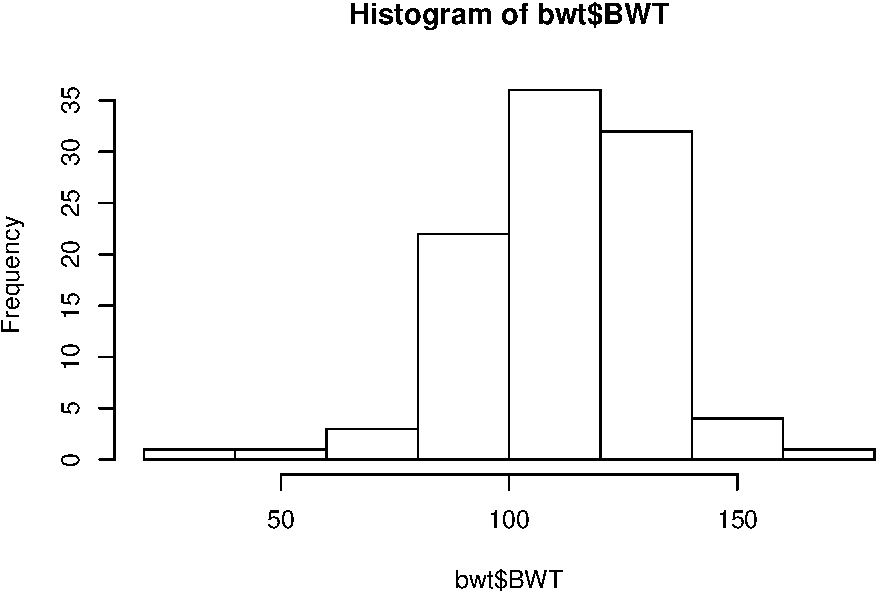
\includegraphics{bst4r_files/figure-latex/unnamed-chunk-46-1.pdf}

\texttt{ggplot2}

\begin{Shaded}
\begin{Highlighting}[]
\KeywordTok{library}\NormalTok{(ggplot2)}
 \KeywordTok{ggplot}\NormalTok{(}\DataTypeTok{data =}\NormalTok{ bwt,}\KeywordTok{aes}\NormalTok{(BWT))}\OperatorTok{+}
\StringTok{  }\KeywordTok{geom_histogram}\NormalTok{(}\DataTypeTok{fill =} \StringTok{"white"}\NormalTok{, }\DataTypeTok{color =} \StringTok{"black"}\NormalTok{,}\DataTypeTok{binwidth =} \DecValTok{10}\NormalTok{)}\OperatorTok{+}
\StringTok{  }\KeywordTok{ylab}\NormalTok{(}\StringTok{"Count"}\NormalTok{)}
\end{Highlighting}
\end{Shaded}

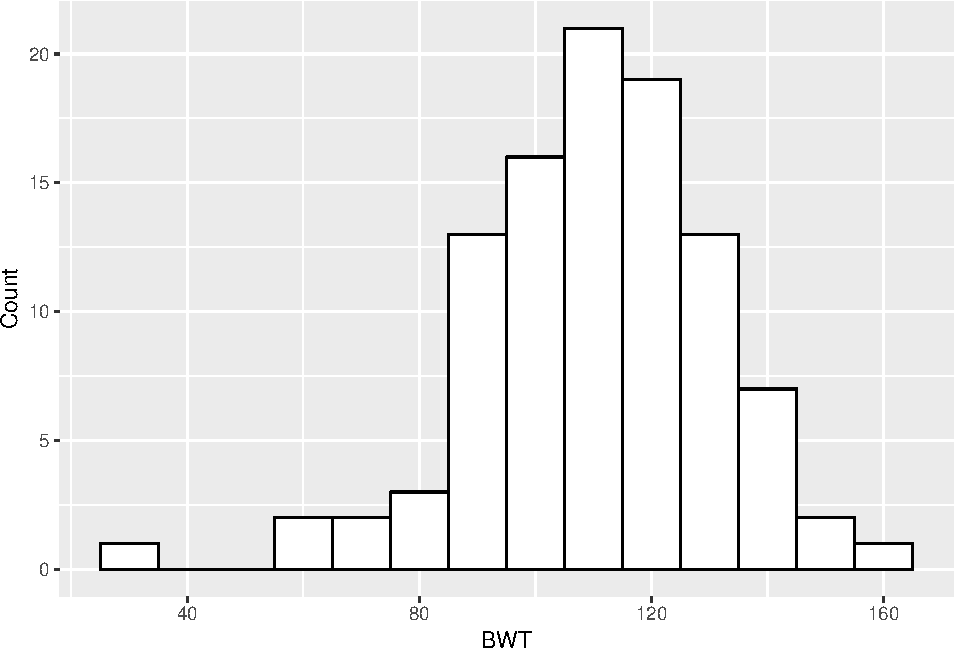
\includegraphics{bst4r_files/figure-latex/unnamed-chunk-47-1.pdf}

\hypertarget{stem-and-leaf-plots}{%
\subsubsection{Stem-and-Leaf Plots}\label{stem-and-leaf-plots}}

Base-R

\begin{Shaded}
\begin{Highlighting}[]
\KeywordTok{stem}\NormalTok{(bwt}\OperatorTok{$}\NormalTok{BWT, }\DataTypeTok{scale =} \DecValTok{2}\NormalTok{)}
\end{Highlighting}
\end{Shaded}

\begin{verbatim}

  The decimal point is 1 digit(s) to the right of the |

   3 | 2
   4 | 
   5 | 8
   6 | 478
   7 | 
   8 | 3556788999
   9 | 12344568889
  10 | 0123444445567888899
  11 | 00122235555556889
  12 | 01112222344445567788
  13 | 222334557888
  14 | 0146
  15 | 5
  16 | 1
\end{verbatim}

\hypertarget{box-plots}{%
\subsubsection{Box Plots}\label{box-plots}}

Base-R

\begin{Shaded}
\begin{Highlighting}[]
\KeywordTok{boxplot}\NormalTok{(bwt}\OperatorTok{$}\NormalTok{BWT)}
\end{Highlighting}
\end{Shaded}

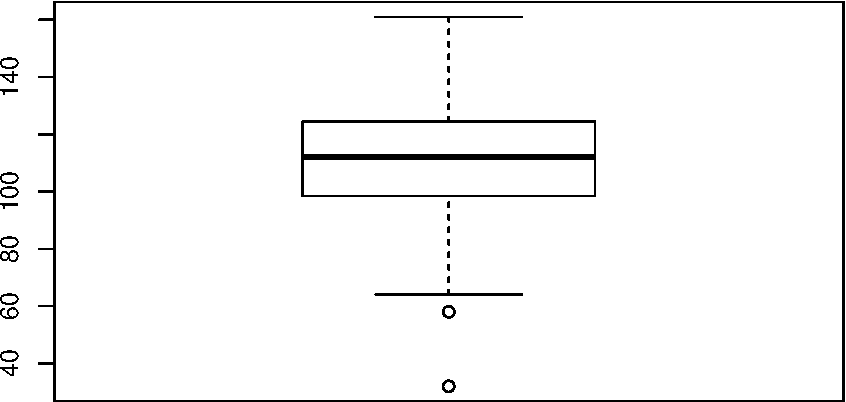
\includegraphics{bst4r_files/figure-latex/unnamed-chunk-49-1.pdf}

\texttt{ggplot2}

\begin{Shaded}
\begin{Highlighting}[]
\KeywordTok{ggplot}\NormalTok{(bwt, }\KeywordTok{aes}\NormalTok{(}\DataTypeTok{x =} \StringTok{""}\NormalTok{,BWT))}\OperatorTok{+}\KeywordTok{geom_boxplot}\NormalTok{()}
\end{Highlighting}
\end{Shaded}

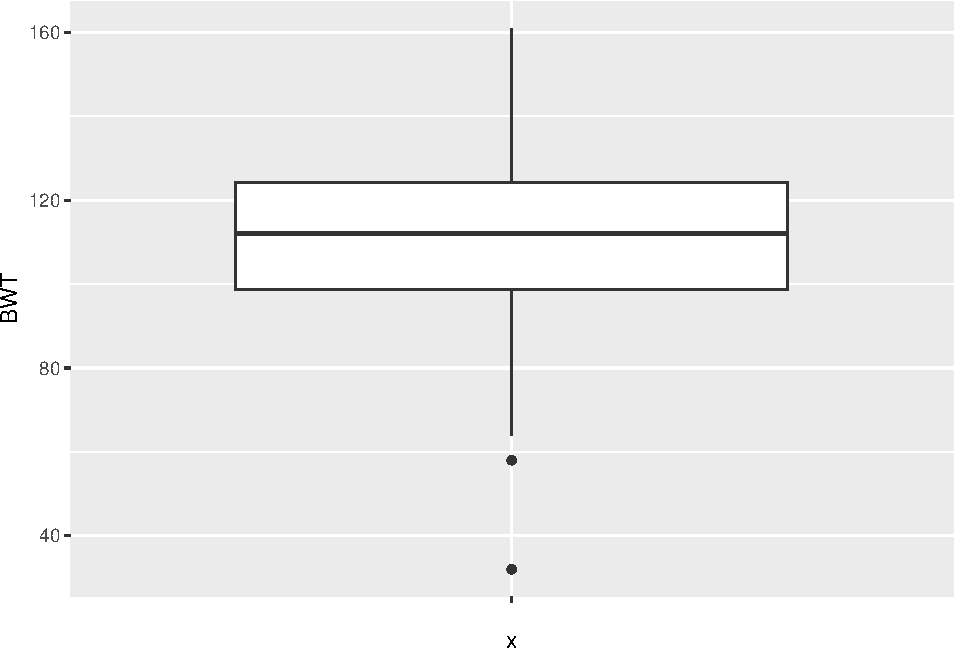
\includegraphics{bst4r_files/figure-latex/unnamed-chunk-50-1.pdf}

\hypertarget{probability}{%
\section{Probability}\label{probability}}

The probability of an event is the relative frequency of an event
(outcome) within a sample space (all possible outcomes).

\hypertarget{some-useful-probabilistic-notation}{%
\subsubsection{Some Useful Probabilistic
notation}\label{some-useful-probabilistic-notation}}

\begin{longtable}[]{@{}cl@{}}
\toprule
Symbol & Definition\tabularnewline
\midrule
\endhead
&\tabularnewline
\(\cap\) & intersection (and)\tabularnewline
\(\cup\) & union (or)\tabularnewline
A' \(\bar{A}\) \(A^c\) & complement (not)\tabularnewline
\{ \} & event\tabularnewline
\(Pr(A)\) & Probability that event A will occur.\tabularnewline
\(Pr(A\|B)\) & The probability of A occurring if B
occurred.\tabularnewline
\(P(A')\) & The probability A will not occur.
(\(\bar{A}=1-Pr(A)\))\tabularnewline
\(Pr(A\cap B)\) & The Probability events A and B occurring
together.\tabularnewline
\(Pr(A\cup B)\) & Probability events either A or B occur, or they both
occurr.\tabularnewline
\bottomrule
\end{longtable}

\begin{enumerate}
\def\labelenumi{\arabic{enumi}.}
\tightlist
\item
  The probability of an event (\(Pr(E)\)) always satisfies:
  \[0 \leq \text{Pr(E)} \leq 1\]
\item
  If events A and B cannot both occur simultanously, they are
  \textbf{mutually exclusive}. \[Pr(A\cap B)=0\]
\item
  Two events A and B are called independent if
  \[Pr(A\ycap B)=Pr(A)\times Pr(B)\]
\item
  Two events A and B are called dependent if
  \[Pr(A\cap B)\ne Pr(A)\times Pr(B)\]
\end{enumerate}

\hypertarget{laws-of-probability}{%
\subsection{Laws of Probability}\label{laws-of-probability}}

\hypertarget{the-multiplication-law-of-probability-pracap-b}{%
\subsubsection{\texorpdfstring{The Multiplication Law of Probability:
\(Pr(A\cap B)\)}{The Multiplication Law of Probability: Pr(A\textbackslash{}cap B)}}\label{the-multiplication-law-of-probability-pracap-b}}

If \(A_1,...,A_n\) are mutually independent events, then
\[Pr(A_1 \cap A_2 \cap ... \cap A_n) = Pr(A_1)\times Pr(A_2)\times ...\times Pr(A_n)\]

\hypertarget{the-addition-law-of-probability-pracup-b}{%
\subsubsection{\texorpdfstring{The Addition Law of Probability:
\(Pr(A\cup B)\)}{The Addition Law of Probability: Pr(A\textbackslash{}cup B)}}\label{the-addition-law-of-probability-pracup-b}}

If \(A\text{ and }B\) are \textbf{any} events, then
\[Pr(A \cup B) = Pr(A)+ Pr(B)- Pr(A\cap B)\]

If \(A\text{ and }B\) are \textbf{mutually exclusive}, then
\[Pr(A \cup B) = Pr(A)+ Pr(B)\]

If \(A\text{ and }B\) are \textbf{independent} events, then
\[Pr(A \cup B) = Pr(A)+ Pr(B)\times[1-Pr(A)]\]

\hypertarget{conditional-probability}{%
\subsection{Conditional Probability}\label{conditional-probability}}

A conditional probability is the probability of one event if another
event occurred. \[Pr(A|B) = \frac{Pr(A\cap B)}{Pr(A)}\]

\begin{enumerate}
\def\labelenumi{\arabic{enumi}.}
\tightlist
\item
  If A and B are independent events, then
  \[Pr(B|A) = Pr(B) = Pr(B|\bar{A})\]
\item
  If two events A and B are dependent, then
  \[Pr(B|A)\ne Pr(B) \ne Pr(B|\bar{A})\] and
  \[Pr(A\cap B) \ne Pr(A)\times Pr(B)\]
\end{enumerate}

\hypertarget{relative-risk}{%
\subsubsection{Relative Risk}\label{relative-risk}}

The relative risk (RR) of B given is
\[RR=\frac{Pr(B|A)}{Pr(B|\bar{A})}\]

If two events A and B are independent, then RR = 1.

\hypertarget{total-probability}{%
\subsubsection{Total Probability}\label{total-probability}}

Let A

\hypertarget{bayes-rule-and-screening-tests}{%
\subsection{Bayes' Rule and Screening
Tests}\label{bayes-rule-and-screening-tests}}

\hypertarget{bayesian-inference}{%
\subsection{Bayesian inference}\label{bayesian-inference}}

\hypertarget{roc-curves}{%
\subsection{RoC Curves}\label{roc-curves}}

\hypertarget{prevalence-and-incidence}{%
\subsection{Prevalence and incidence}\label{prevalence-and-incidence}}

\hypertarget{discrete-probability-distributions}{%
\section{Discrete Probability
distributions}\label{discrete-probability-distributions}}

\hypertarget{introduction}{%
\subsection{Introduction}\label{introduction}}

\hypertarget{random-variables}{%
\subsection{Random Variables}\label{random-variables}}

\hypertarget{the-probability-mass-function-for-a-discrete-random-variable}{%
\subsection{The Probability-Mass Function for a Discrete Random
Variable}\label{the-probability-mass-function-for-a-discrete-random-variable}}

\hypertarget{the-expected-value-of-a-discrete-random-variable}{%
\subsection{The Expected Value of a discrete Random
Variable}\label{the-expected-value-of-a-discrete-random-variable}}

\hypertarget{the-variance-of-a-discrete-random-variable}{%
\subsection{The Variance of a Discrete Random
Variable}\label{the-variance-of-a-discrete-random-variable}}

\hypertarget{the-cumulative-distribution-function-of-a-discrete-random-variable}{%
\subsection{The Cumulative-Distribution Function of a Discrete Random
Variable}\label{the-cumulative-distribution-function-of-a-discrete-random-variable}}

\hypertarget{permutations-and-combinations}{%
\subsection{Permutations and
Combinations}\label{permutations-and-combinations}}

\hypertarget{the-binomial-distribution}{%
\subsection{The Binomial distribution}\label{the-binomial-distribution}}

\hypertarget{expected-value-and-variance-of-the-binomial-distribution}{%
\subsection{Expected Value and Variance of the Binomial
distribution}\label{expected-value-and-variance-of-the-binomial-distribution}}

\hypertarget{the-poisson-distribution}{%
\subsection{The Poisson distribution}\label{the-poisson-distribution}}

\hypertarget{computation-of-poisson-probabilities}{%
\subsection{Computation of Poisson
Probabilities}\label{computation-of-poisson-probabilities}}

\hypertarget{expected-value-and-variance-of-the-poisson-distribution}{%
\subsection{Expected Value and Variance of the Poisson
Distribution}\label{expected-value-and-variance-of-the-poisson-distribution}}

\hypertarget{poisson-approximation-to-the-binomial-distribution}{%
\subsection{Poisson Approximation to the Binomial
Distribution}\label{poisson-approximation-to-the-binomial-distribution}}

\hypertarget{continuous-probability-distributions}{%
\section{Continuous Probability
distributions}\label{continuous-probability-distributions}}

\hypertarget{introduction-1}{%
\subsection{Introduction}\label{introduction-1}}

\hypertarget{general-concepts}{%
\subsection{General Concepts}\label{general-concepts}}

\hypertarget{the-normal-distribution}{%
\subsection{The Normal Distribution}\label{the-normal-distribution}}

\hypertarget{properties-of-the-standard-normal-distribution}{%
\subsection{Properties of the Standard Normal
Distribution}\label{properties-of-the-standard-normal-distribution}}

\hypertarget{conversion-from-an-n2-distribution-to-an-n-01-distribution}{%
\subsection{Conversion from an n(μ,σ2) Distribution to an n (0,1)
Distribution}\label{conversion-from-an-n2-distribution-to-an-n-01-distribution}}

\hypertarget{linear-combinations-of-random-variables}{%
\subsection{Linear Combinations of Random
Variables}\label{linear-combinations-of-random-variables}}

\hypertarget{normal-approximation-to-the-binomial-distribution}{%
\subsection{Normal Approximation to the Binomial
Distribution}\label{normal-approximation-to-the-binomial-distribution}}

\hypertarget{normal-approximation-to-the-poisson-distribution}{%
\subsection{Normal Approximation to the Poisson
Distribution}\label{normal-approximation-to-the-poisson-distribution}}

\hypertarget{estimation}{%
\section{Estimation}\label{estimation}}

\hypertarget{introduction-2}{%
\subsection{Introduction}\label{introduction-2}}

\hypertarget{the-relationship-between-population-and-sample}{%
\subsection{The Relationship Between Population and
Sample}\label{the-relationship-between-population-and-sample}}

\hypertarget{random-number-tables}{%
\subsection{Random-Number Tables}\label{random-number-tables}}

\hypertarget{randomized-clinical-trials}{%
\subsection{Randomized Clinical
Trials}\label{randomized-clinical-trials}}

\hypertarget{estimation-of-the-mean-of-a-distribution}{%
\subsection{Estimation of the Mean of a
Distribution}\label{estimation-of-the-mean-of-a-distribution}}

\hypertarget{estimation-of-the-variance-of-a-distribution}{%
\subsection{Estimation of the Variance of a
Distribution}\label{estimation-of-the-variance-of-a-distribution}}

\hypertarget{estimation-for-the-binomial-distribution}{%
\subsection{Estimation for the Binomial
Distribution}\label{estimation-for-the-binomial-distribution}}

\hypertarget{estimation-for-the-poisson-distribution}{%
\subsection{Estimation for the Poisson
Distribution}\label{estimation-for-the-poisson-distribution}}

\hypertarget{one-sided-confidence-intervals}{%
\subsection{One-Sided Confidence
Intervals}\label{one-sided-confidence-intervals}}

\hypertarget{the-bootstrap}{%
\subsection{The Bootstrap}\label{the-bootstrap}}

\hypertarget{hypothesis-testing-one-sample-inference}{%
\section{hypothesis testing: one-Sample
inference}\label{hypothesis-testing-one-sample-inference}}

\hypertarget{introduction-3}{%
\subsection{introduction}\label{introduction-3}}

\hypertarget{general-concepts-1}{%
\subsection{General Concepts}\label{general-concepts-1}}

\hypertarget{one-sample-test-for-the-mean-of-a-normal-distribution-one-sided-alternatives}{%
\subsection{one-Sample test for the Mean of a normal distribution:
one-Sided
Alternatives}\label{one-sample-test-for-the-mean-of-a-normal-distribution-one-sided-alternatives}}

\hypertarget{one-sample-test-for-the-mean-of-a-normal-distribution-two-sided-alternatives}{%
\subsection{one-Sample test for the Mean of a normal distribution:
two-Sided
Alternatives}\label{one-sample-test-for-the-mean-of-a-normal-distribution-two-sided-alternatives}}

\hypertarget{the-relationship-between-hypothesis-testing-and-confidence-intervals}{%
\subsection{the Relationship Between hypothesis testing and Confidence
intervals}\label{the-relationship-between-hypothesis-testing-and-confidence-intervals}}

\hypertarget{the-power-of-a-test}{%
\subsection{the Power of a test}\label{the-power-of-a-test}}

\hypertarget{sample-size-determination}{%
\subsection{Sample-Size determination}\label{sample-size-determination}}

\hypertarget{one-sample-2-test-for-the-variance-of-a-normal-distribution}{%
\subsection{one-Sample χ2 test for the Variance of a normal
distribution}\label{one-sample-2-test-for-the-variance-of-a-normal-distribution}}

\hypertarget{one-sample-inference-for-the-binomial-distribution}{%
\subsection{one-Sample inference for the Binomial
distribution}\label{one-sample-inference-for-the-binomial-distribution}}

\hypertarget{one-sample-inference-for-the-poisson-distribution}{%
\subsection{one-Sample inference for the Poisson
distribution}\label{one-sample-inference-for-the-poisson-distribution}}

\hypertarget{hypothesis-testing-two-sample-inference}{%
\section{Hypothesis Testing: two-Sample
inference}\label{hypothesis-testing-two-sample-inference}}

\hypertarget{introduction-4}{%
\subsection{introduction}\label{introduction-4}}

\hypertarget{the-paired-t-test}{%
\subsection{the Paired t test}\label{the-paired-t-test}}

\hypertarget{interval-estimation-for-the-comparison-of-means-from-two-paired-samples}{%
\subsection{interval Estimation for the Comparison of Means from two
Paired
Samples}\label{interval-estimation-for-the-comparison-of-means-from-two-paired-samples}}

\hypertarget{two-sample-t-test-for-independent-samples-with-equal-variances}{%
\subsection{two-Sample t test for independent Samples with Equal
Variances}\label{two-sample-t-test-for-independent-samples-with-equal-variances}}

\hypertarget{interval-estimation-for-the-comparison-of-means-from-two-independent-samples-equal-variance-case}{%
\subsection{interval Estimation for the Comparison of Means from two
independent Samples (Equal Variance
Case)}\label{interval-estimation-for-the-comparison-of-means-from-two-independent-samples-equal-variance-case}}

\hypertarget{testing-for-the-equality-of-two-variances}{%
\subsection{testing for the Equality of two
Variances}\label{testing-for-the-equality-of-two-variances}}

\hypertarget{two-sample-t-test-for-independent-samples-with-unequal-variances}{%
\subsection{two-Sample t test for independent Samples with Unequal
Variances}\label{two-sample-t-test-for-independent-samples-with-unequal-variances}}

\hypertarget{estimation-of-sample-size-and-power-for-comparing-two-means}{%
\subsection{Estimation of Sample Size and Power for Comparing two
Means}\label{estimation-of-sample-size-and-power-for-comparing-two-means}}

\hypertarget{the-treatment-of-outliers}{%
\subsection{the treatment of outliers}\label{the-treatment-of-outliers}}

\hypertarget{derivation-of-equation-8.13}{%
\subsection{derivation of Equation
8.13}\label{derivation-of-equation-8.13}}

\hypertarget{nonparametric-methods}{%
\section{Nonparametric Methods}\label{nonparametric-methods}}

\hypertarget{introduction-5}{%
\subsection{introduction}\label{introduction-5}}

\hypertarget{the-sign-test}{%
\subsection{the Sign test}\label{the-sign-test}}

\hypertarget{the-wilcoxon-signed-rank-test}{%
\subsection{the Wilcoxon Signed-Rank
test}\label{the-wilcoxon-signed-rank-test}}

\hypertarget{the-wilcoxon-rank-sum-test}{%
\subsection{the Wilcoxon Rank-Sum
test}\label{the-wilcoxon-rank-sum-test}}

\hypertarget{permutation-tests}{%
\subsection{Permutation tests}\label{permutation-tests}}

\hypertarget{hypothesis-testingcategoricaldata}{%
\section{hypothesis
testing:Categoricaldata}\label{hypothesis-testingcategoricaldata}}

\hypertarget{introduction-6}{%
\subsection{introduction}\label{introduction-6}}

\hypertarget{two-sample-test-for-binomial-proportions}{%
\subsection{two-Sample test for Binomial
Proportions}\label{two-sample-test-for-binomial-proportions}}

\hypertarget{fishers-exact-test}{%
\subsection{Fisher's Exact test}\label{fishers-exact-test}}

\hypertarget{two-sample-test-for-binomial-proportions-for-matched-pair-data-mcnemars-test}{%
\subsection{two-Sample test for Binomial Proportions for Matched-Pair
data (Mcnemar's
test)}\label{two-sample-test-for-binomial-proportions-for-matched-pair-data-mcnemars-test}}

\hypertarget{estimation-of-sample-size-and-power-for-comparing-two-binomial-proportions}{%
\subsection{Estimation of Sample Size and Power for Comparing two
Binomial
Proportions}\label{estimation-of-sample-size-and-power-for-comparing-two-binomial-proportions}}

\hypertarget{r-c-contingency-tables}{%
\subsection{R × C Contingency tables}\label{r-c-contingency-tables}}

\hypertarget{chi-square-goodness-of-fit-test}{%
\subsection{Chi-Square Goodness-of-Fit
test}\label{chi-square-goodness-of-fit-test}}

\hypertarget{the-kappa-statistic}{%
\subsection{the Kappa Statistic}\label{the-kappa-statistic}}

\hypertarget{derivation-of-selected-formulas}{%
\subsection{derivation of Selected
Formulas}\label{derivation-of-selected-formulas}}

\hypertarget{regression-and-correlation-methods}{%
\section{Regression and Correlation
Methods}\label{regression-and-correlation-methods}}

\hypertarget{introduction-7}{%
\subsection{introduction}\label{introduction-7}}

\hypertarget{general-concepts-2}{%
\subsection{General Concepts}\label{general-concepts-2}}

\hypertarget{fitting-regression-linesthe-method-of-least-squares}{%
\subsection{Fitting Regression Lines---the Method of Least
Squares}\label{fitting-regression-linesthe-method-of-least-squares}}

\hypertarget{inferences-about-parameters-from-regression-lines}{%
\subsection{inferences About Parameters from Regression
Lines}\label{inferences-about-parameters-from-regression-lines}}

\hypertarget{interval-estimation-for-linear-regression}{%
\subsection{interval Estimation for Linear
Regression}\label{interval-estimation-for-linear-regression}}

\hypertarget{assessing-the-goodness-of-fit-of-regression-lines}{%
\subsection{Assessing the Goodness of Fit of Regression
Lines}\label{assessing-the-goodness-of-fit-of-regression-lines}}

\hypertarget{the-correlation-coefficient}{%
\subsection{the Correlation
Coefficient}\label{the-correlation-coefficient}}

\hypertarget{statistical-inference-for-correlation-coefficients}{%
\subsection{Statistical inference for Correlation
Coefficients}\label{statistical-inference-for-correlation-coefficients}}

\hypertarget{multiple-regression}{%
\subsection{Multiple Regression}\label{multiple-regression}}

\hypertarget{partial-and-multiple-correlation}{%
\subsection{Partial and Multiple
Correlation}\label{partial-and-multiple-correlation}}

\hypertarget{rank-correlation}{%
\subsection{Rank Correlation}\label{rank-correlation}}

\hypertarget{interval-estimation-for-rank-correlation-coefficients}{%
\subsection{interval Estimation for Rank-Correlation
Coefficients}\label{interval-estimation-for-rank-correlation-coefficients}}

\hypertarget{derivation-of-equation-11.26}{%
\subsection{derivation of Equation
11.26}\label{derivation-of-equation-11.26}}

\hypertarget{multisample-inference}{%
\section{Multisample inference}\label{multisample-inference}}

\hypertarget{introduction-to-the-one-way-analysis-of-variance}{%
\subsection{introduction to the one-Way Analysis of
Variance}\label{introduction-to-the-one-way-analysis-of-variance}}

\hypertarget{one-way-anovafixed-effects-model}{%
\subsection{one-Way AnoVA---Fixed-Effects
Model}\label{one-way-anovafixed-effects-model}}

\hypertarget{hypothesis-testing-in-one-way-anova-fixed-effects-model}{%
\subsection{hypothesis testing in one-Way AnoVA--- Fixed-Effects
Model}\label{hypothesis-testing-in-one-way-anova-fixed-effects-model}}

\hypertarget{comparisons-of-specific-groups-in-one--way-anova}{%
\subsection{Comparisons of Specific Groups in one- Way
AnoVA}\label{comparisons-of-specific-groups-in-one--way-anova}}

\hypertarget{two-way-anova}{%
\subsection{two-Way AnoVA}\label{two-way-anova}}

\hypertarget{the-kruskal-wallis-test}{%
\subsection{the Kruskal-Wallis test}\label{the-kruskal-wallis-test}}

\hypertarget{one-way-anovathe-random-effects-model}{%
\subsection{one-Way AnoVA---the Random-Effects
Model}\label{one-way-anovathe-random-effects-model}}

\hypertarget{the-intraclass-correlation-coefficient}{%
\subsection{the intraclass Correlation
Coefficient}\label{the-intraclass-correlation-coefficient}}

\hypertarget{mixed-models}{%
\subsection{Mixed Models}\label{mixed-models}}

\hypertarget{derivation-of-equation}{%
\subsection{derivation of Equation}\label{derivation-of-equation}}

\hypertarget{design-and-analysis-techniques-for-epidemiologic-studies}{%
\section{design and Analysis techniques for Epidemiologic
Studies}\label{design-and-analysis-techniques-for-epidemiologic-studies}}

\hypertarget{introduction-8}{%
\subsection{introduction}\label{introduction-8}}

\hypertarget{study-design}{%
\subsection{Study design}\label{study-design}}

\hypertarget{measures-of-effect-for-categorical-data}{%
\subsection{Measures of Effect for Categorical
data}\label{measures-of-effect-for-categorical-data}}

\hypertarget{attributable-risk}{%
\subsection{Attributable Risk}\label{attributable-risk}}

\hypertarget{confounding-and-standardization}{%
\subsection{Confounding and
Standardization}\label{confounding-and-standardization}}

\hypertarget{methods-of-inference-for-stratified-categorical-datathe-mantel-haenszel-test}{%
\subsection{Methods of inference for Stratified Categorical data---the
Mantel-haenszel
test}\label{methods-of-inference-for-stratified-categorical-datathe-mantel-haenszel-test}}

\hypertarget{multiple-logistic-regression}{%
\subsection{Multiple Logistic
Regression}\label{multiple-logistic-regression}}

\hypertarget{extensions-to-logistic-regression}{%
\subsection{Extensions to Logistic
Regression}\label{extensions-to-logistic-regression}}

\hypertarget{sample-size-estimation-for-logistic-regression}{%
\subsection{Sample Size Estimation for Logistic
Regression}\label{sample-size-estimation-for-logistic-regression}}

\hypertarget{meta-analysis}{%
\subsection{Meta-Analysis}\label{meta-analysis}}

\hypertarget{equivalence-studies}{%
\subsection{Equivalence Studies}\label{equivalence-studies}}

\hypertarget{the-cross-over-design}{%
\subsection{the Cross-over design}\label{the-cross-over-design}}

\hypertarget{clustered-binary-data}{%
\subsection{Clustered Binary data}\label{clustered-binary-data}}

\hypertarget{longitudinal-data-analysis}{%
\subsection{Longitudinal data
Analysis}\label{longitudinal-data-analysis}}

\hypertarget{measurement-error-methods}{%
\subsection{Measurement-Error Methods}\label{measurement-error-methods}}

\hypertarget{missing-data}{%
\subsection{Missing data}\label{missing-data}}

\hypertarget{derivation-of-100-1--ci-for-the-risk-difference}{%
\subsection{derivation of 100\% × (1 -- α) Ci for the Risk
difference}\label{derivation-of-100-1--ci-for-the-risk-difference}}

\hypertarget{hypothesis-testing-person-time-data}{%
\section{Hypothesis testing: Person-time
data}\label{hypothesis-testing-person-time-data}}

\hypertarget{measure-of-effect-for-person-time-data}{%
\subsection{Measure of Effect for Person-time
data}\label{measure-of-effect-for-person-time-data}}

\hypertarget{one-sample-inference-for-incidence-rate-data}{%
\subsection{one-Sample inference for incidence-Rate
data}\label{one-sample-inference-for-incidence-rate-data}}

\hypertarget{two-sample-inference-for-incidence-rate-data}{%
\subsection{two-Sample inference for incidence-Rate
data}\label{two-sample-inference-for-incidence-rate-data}}

\hypertarget{power-and-sample-size-estimation-for-person-time-data}{%
\subsection{Power and Sample-Size Estimation for Person-time
data}\label{power-and-sample-size-estimation-for-person-time-data}}

\hypertarget{inference-for-stratified-person-time-data}{%
\subsection{Inference for Stratified Person-Time
Data}\label{inference-for-stratified-person-time-data}}

\hypertarget{power-and-sample-size-estimation-for-stratified-person-time-data}{%
\subsection{Power and Sample-Size Estimation for Stratified Person-Time
Data}\label{power-and-sample-size-estimation-for-stratified-person-time-data}}

\hypertarget{testing-for-trend-incidence-rate-data}{%
\subsection{Testing for Trend: Incidence-Rate
Data}\label{testing-for-trend-incidence-rate-data}}

\hypertarget{introduction-to-survival-analysis}{%
\subsection{Introduction to Survival
Analysis}\label{introduction-to-survival-analysis}}

\hypertarget{estimation-of-survival-curves-the-kaplan-meier-estimator}{%
\subsection{Estimation of Survival Curves: The Kaplan-Meier
Estimator}\label{estimation-of-survival-curves-the-kaplan-meier-estimator}}

\hypertarget{the-log-rank-test}{%
\subsection{The Log-Rank Test}\label{the-log-rank-test}}

\hypertarget{the-proportional-hazards-model}{%
\subsection{The Proportional-Hazards
Model}\label{the-proportional-hazards-model}}

\hypertarget{power-and-sample-size-estimation-under-the-proportional-hazards-model}{%
\subsection{Power and Sample-Size Estimation under the
Proportional-Hazards
Model}\label{power-and-sample-size-estimation-under-the-proportional-hazards-model}}

\hypertarget{parametric-survival-analysis}{%
\subsection{Parametric Survival
Analysis}\label{parametric-survival-analysis}}

\hypertarget{parametric-regression-models-for-survival-data}{%
\subsection{Parametric Regression Models for Survival
Data}\label{parametric-regression-models-for-survival-data}}

\hypertarget{derivation-of-selected-formulas-1}{%
\subsection{Derivation of Selected
Formulas}\label{derivation-of-selected-formulas-1}}

\bibliography{book.bib,packages.bib}


\end{document}
